\documentclass{article}
\usepackage[utf8]{inputenc}
\setlength{\parskip}{1em}


\title{Chapter 3}
\author{Jonathan S. Abrahams }
\date{October 2019}

\usepackage{natbib}
\usepackage{graphicx}

\begin{document}

\maketitle

\section{Introduction}
There is a theory which states that if ever anyone discovers exactly what the Universe is for and why it is here, it will instantly disappear and be replaced by something even more bizarre and inexplicable.
There is another theory which states that this has already happened.

\begin{figure}[h!]
\centering
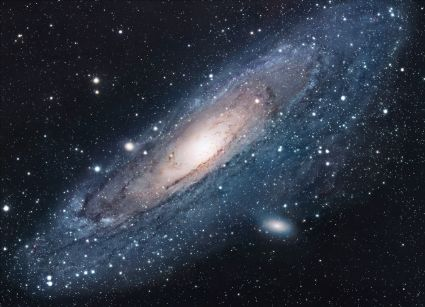
\includegraphics[scale=1.7]{universe}
\caption{The Universe}
\label{fig:universe}
\end{figure}

\section{Methods}
``I always thought something was fundamentally wrong with the universe'' \citep{adams1995hitchhiker}
\section{Results}

\newcommand{\quickwordcount}[1]{%
  \immediate\write18{texcount -1 -sum -merge -q #1.tex output.bbl > #1-words.sum }%
  \input{#1-words.sum} words%
}
There is a plethora of tools to undertake GWAS in both eukaryotic and prokaryotic organisms, most tools are based on detecting SNVs whilst some also analyse the presence or absence of whole genes. However there has been, to our knowledge, no capacity to study structural variants beyond deletions using a GWAS framework. We therefore developed a suite of methods to process SV data into a format that is compatible with GWAS tools and then tested them on a dataset.




\subsection{Structural variations as an effective genotype}


\subsubsection{Read depth based duplications as a genotype for GWAS}

As shown previously, read depth can be a reliable proxy for copy number. Therefore, the previously generated dataset, with a copy number assigned to each gene of each strain, was inputted to pySEER as a matrix. This was possible on pySEER as it can take a binary matrix, intended for the study of pangenomes, as input. However this meant that the CNV data had to be binary and genes with a copy number equal to or less than 1 were set as 0 and genes with a copy number greater than 1 were set to 1.


In order to use SVs as the ‘genotype’ in the ‘genotype-phenotype’ link that GWAS aims to establish, it was first necessary to prove the concept in a proof of concept experiment. In a standard GWAS experiment, phenotypes (such as `MIC $\leq$ 128ug' or `Can metabalise lactose') are often used in a binary format-the outcomes are logged as a zero (0) or one (1). The easiest genotype-phenotype link to discover using GWAS is the 'perfect link' in which a single genotype wholly and consistently is associated with a specific phenotype. To undertake a proof of concept experiment a 'perfect link' phenotype was emulated: the strains containing duplications in Network 1 were given the phenotype of 1 and all other strains were given the phenotype of 0 in this model phenotype. The `genotype' used was the copy number predictions for each gene in each strain.

%The mash data is crap. Likely BPP is in the mix? or perhaps clade 1 vs clade 2 which is unavoidable

\begin{figure}[h!]
\centering
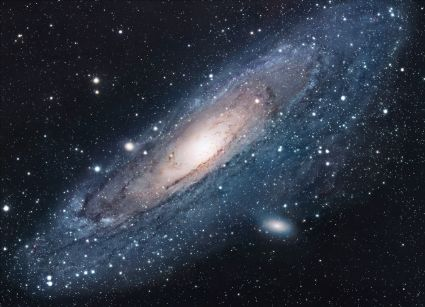
\includegraphics[scale=1.7]{universe}
\caption{Manhatten plot demonstrating a genotype-phenotype link can be established using Duplications and a 'perfect' phenotype. }
\label{fig:Manhatten_1}
\end{figure}



Running a GWAS with the emulated 'perfect link' genotype-phenotype data resulted in the duplicated genes being significantly associated with the 'perfect link' phenotype. Therefore It could be proved that duplications,in principle, could be used as a 'genotype' in GWAS.


Acknowledging the co-existence of all mutation types is imperative in understanding the trajectory evolution is undergoing as neutral mutations can often 'hitch-hike' on mutations which are under positive selection . Therefore analysing a genotype-phenotype link one mutation type at a time may give erroneous results. Our initial analysis of a presence/absence matrix of duplications,whilst functional in a test scenario, would be flawed for use in practise. We therefore sought a rigorous method to provide a holistic genotype, of which all known mutations were inputted, for GWAS in order for a robust genotype-phenotype link to be hypothesised.
%We therefore  used kmers .

\subsection{K-mer based approach as a genotype for GWAS}

The most frequently used method to create a genotype for the analysis of SNVs in GWAS is to split each genome up into overlapping sequence of a specific size (or range of sizes), such sequences are known as 'K-mers' as each sequence is of 'K' size. However this strategy poses a variety of problems for the analysis of SVs in bacteria. 

%How kmers work and why they are useful

The strength and ubiquitous use of K-mers in bioinformatics (refs) stems from the ease K-mers bring to the challenging task of comparing two or more sequences. A K-mer is considered a match to a target sequence only if it is an exact match, therefore avoiding the array of complications stemming from approximate matching of larger sequences. This property is dependent on the length of the kmer and of the variability of the target sequence in addition to other influences. For GWAS,



%Point 1: Structural variations
The length of the repeats involved in recombination-mediated SVs often exceeds the length of K-mers used in GWAS- such mutations are rendered `invisible' to K-mer based GWAS analysis. There are a variety of different solutions to this problem, each with advantages and disadvantages. A seemingly clear solution would be to increase the K-mer length to exceed the length of the repeats of interest which often exceed 1kb in length. The length of K-mers is a balance between sensitivity and specificity,however, and therefore  long (100bp+) K-mers may lead to extremely high specificity (Figure \ref{fig:Sens_spec}). Another strategy is to exclude such repetitive regions, meaning the `pre-repeat' and `post-repeat' sequence are adjacent and thus novel junctions can be captured by regular length K-mers. However, there is evidence that specific IS alleles have different regulatory effects on adjacent genes and thus the exclusion of these sequences. Both strategies were investigated here in order to elucidate the most effective strategy with reference to B.pertussis and more generically, to the bacterial kingdom as a whole.



\begin{figure}[h!]
\centering
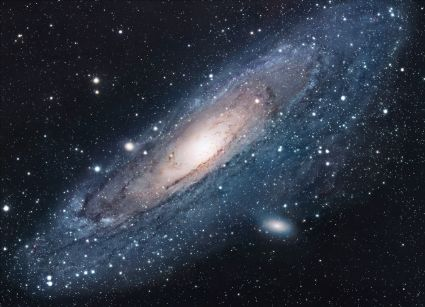
\includegraphics[scale=1.7]{universe}
\caption{Sensitivity and specifcity trade off for K-mer size}
\label{fig:Sens_spec}
\end{figure}


\subsubsection{Ultra-long K-mers overcome the problem}

%Ultra long kmers overcome the problem that kmers are smaller than repeats, however this may not be so applicable to more diverse bacterium outside of B.pertussis.

\subsubsection{Excluding repeat regions overcome the problem}

%Excluding repeat regions was the best solution. However rearangements.

Duplication

\begin{figure}[h!]
\centering
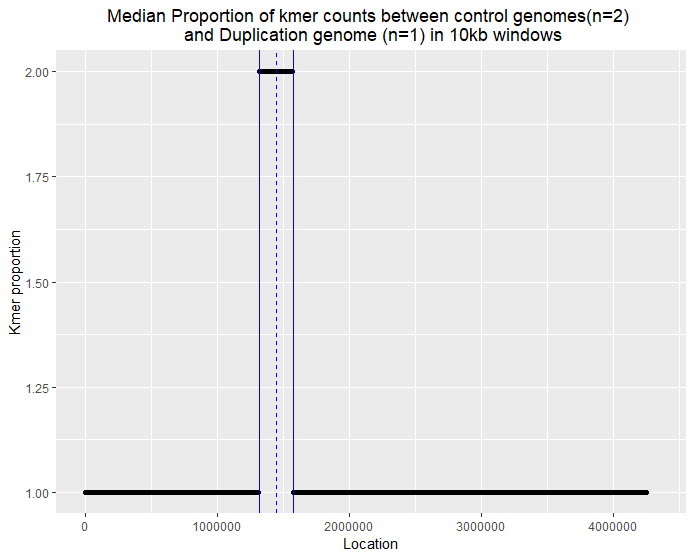
\includegraphics[scale=0.6]{Kmer_dupe.png}
\caption{}
\label{fig:kmer_dupe1}
\end{figure}

PFGE types do not conform to the SNP tree
\begin{figure}[h!]
\centering

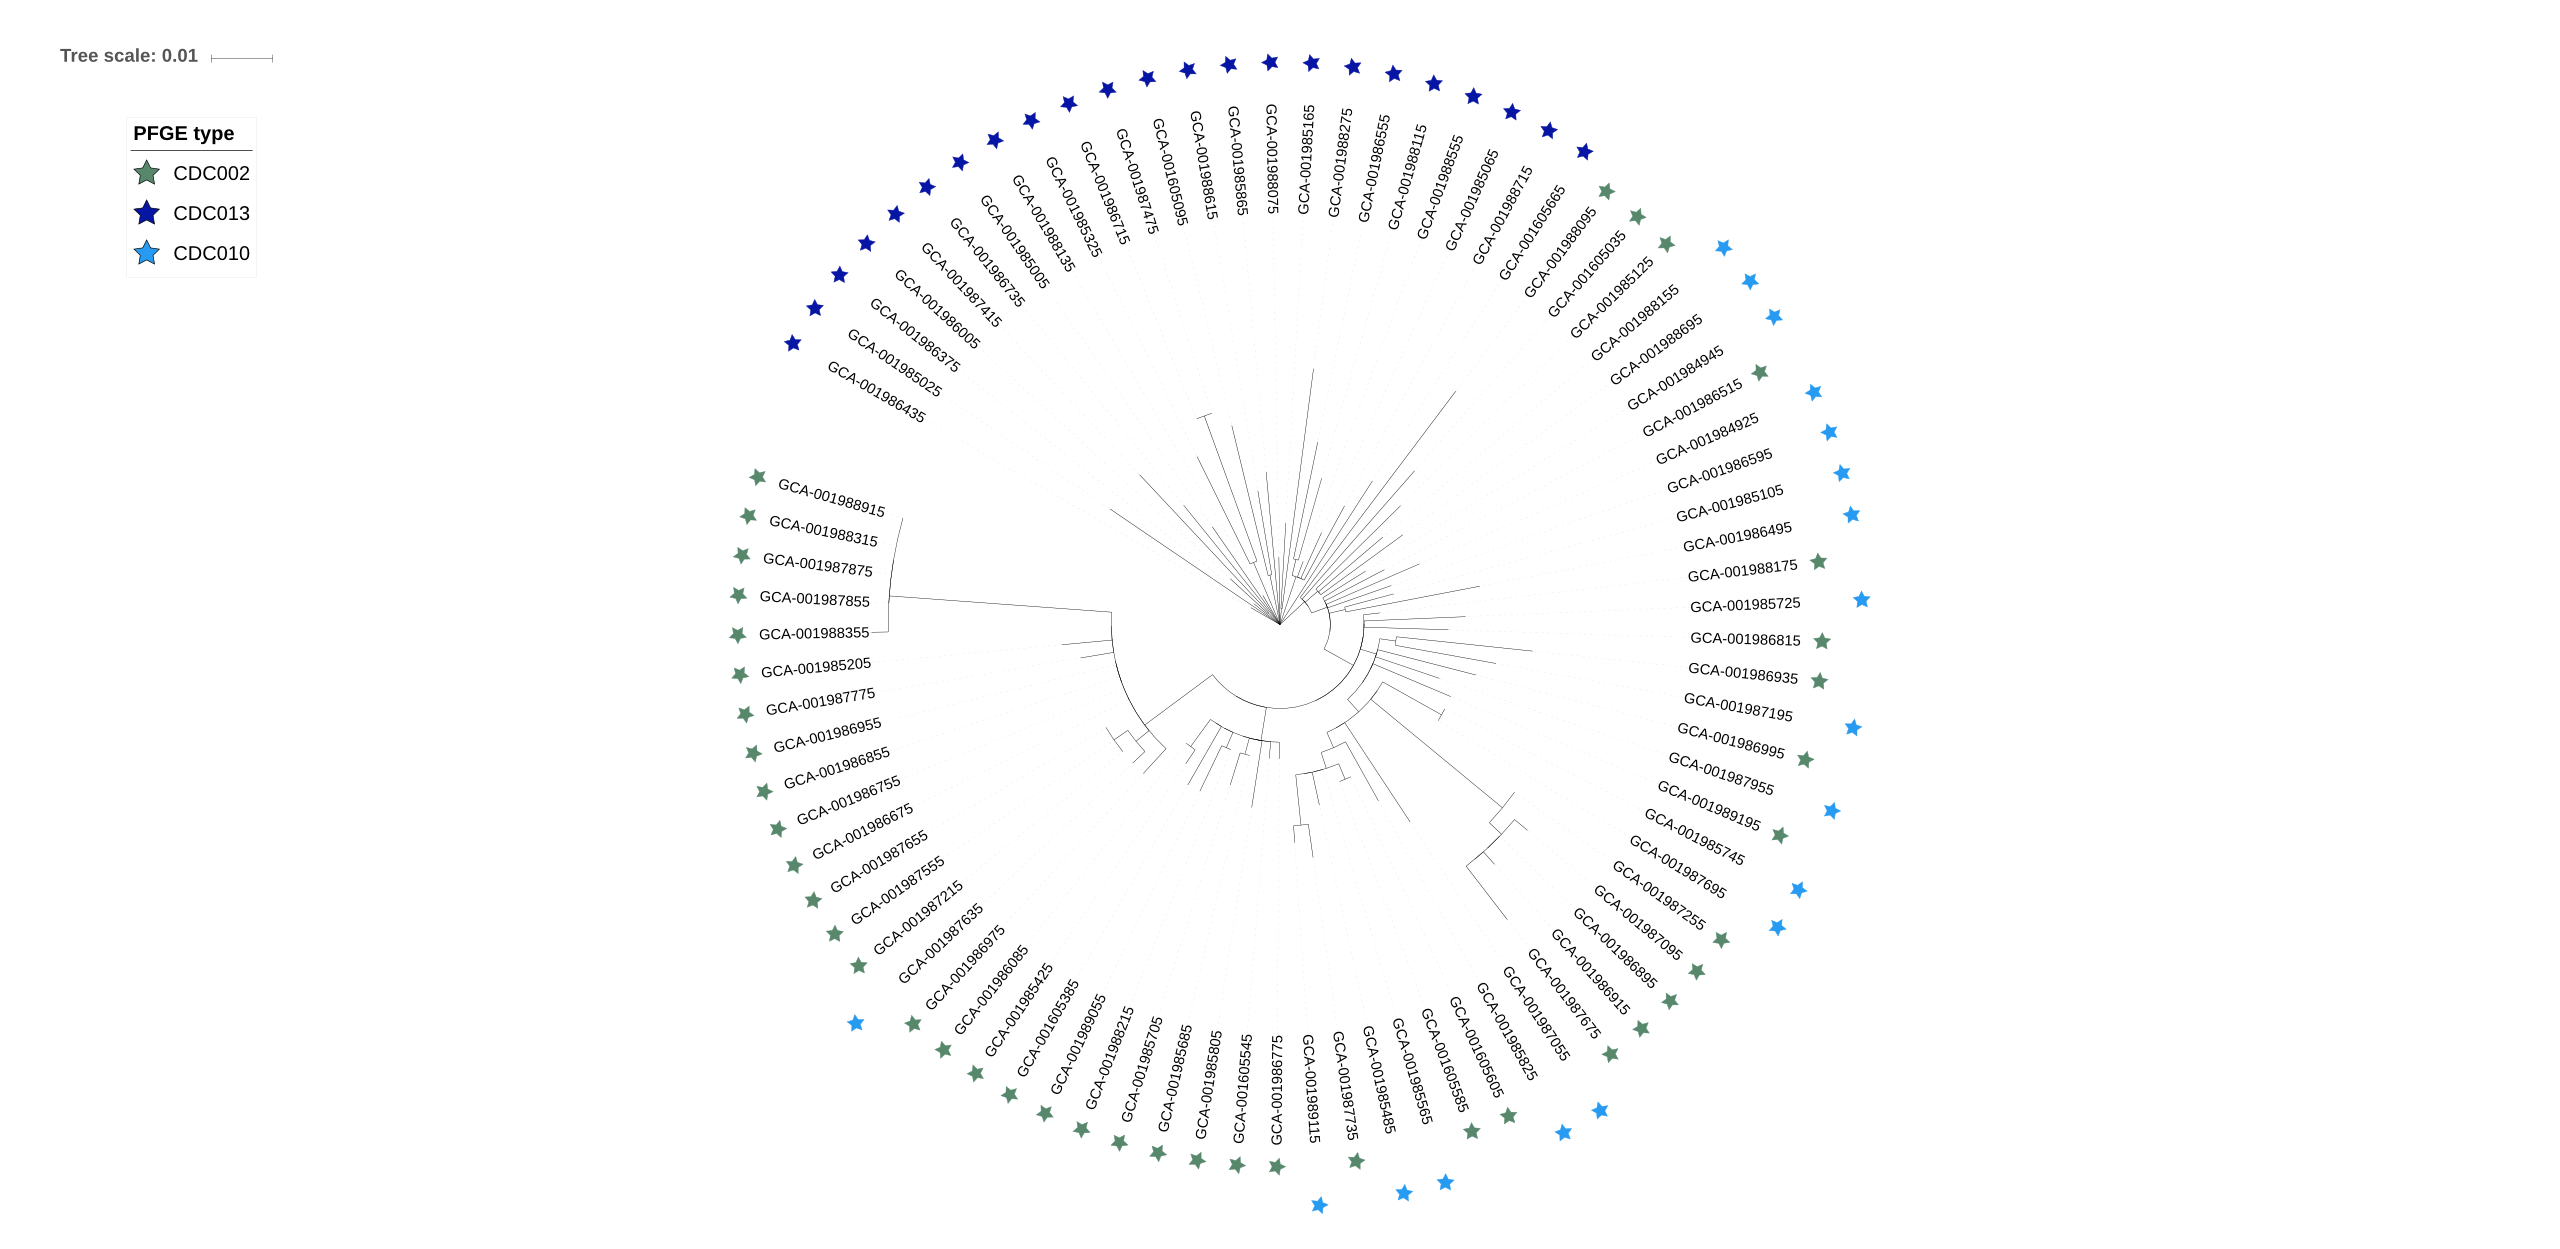
\includegraphics[width=\textwidth{}]{PFGE_tree.png}
\caption{}
\label{fig:PFGE_tree}
\end{figure}


%This figure will be a manhatten plot of this







%\bibliographystyle{plain}
%\bibliography{references}
\end{document}
